% ============================================================
% DIAGRAM: Hebbian Synapse (1949)
% ============================================================
% Caption: Figure 1.2: Hebbian synapse and cell assembly concept.
%          (Adapted from Hebb, 1949, p. 62)
% ============================================================

\documentclass[tikz,border=10pt]{standalone}
\usepackage{tikz}
\usepackage{amsmath}
\usepackage{amsfonts}

\usetikzlibrary{shapes,arrows,positioning,fit,calc,backgrounds}

\begin{document}

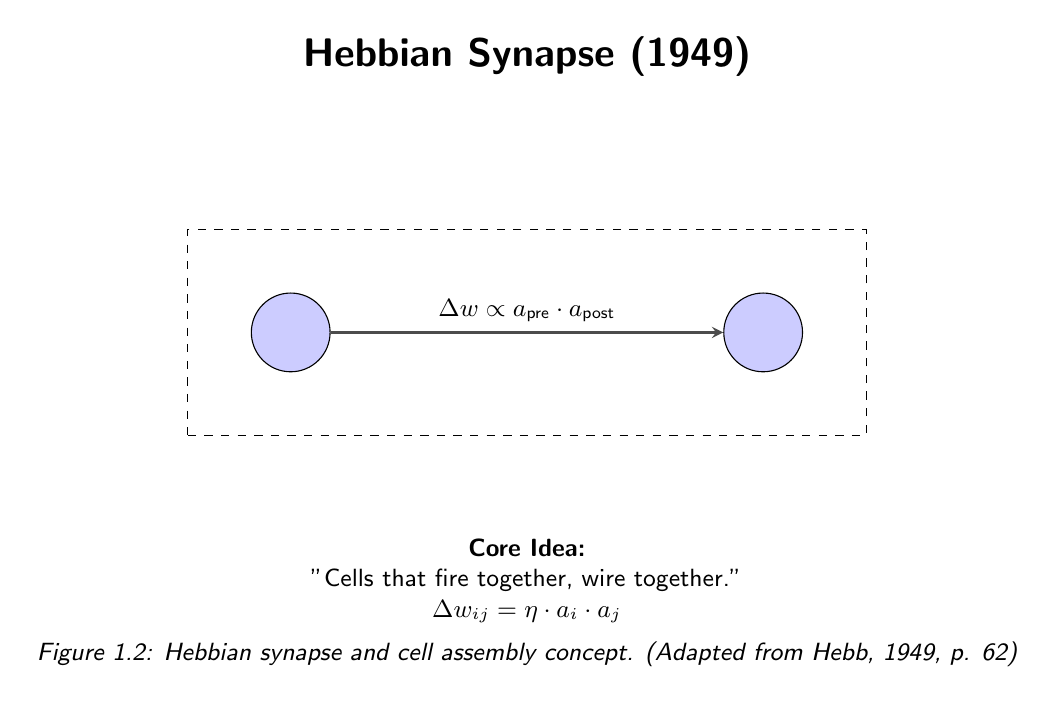
\begin{tikzpicture}[
    neuron/.style={draw, circle, minimum size=1cm, inner sep=0pt, fill=blue!20},
    synapse/.style={draw, circle, minimum size=0.6cm, inner sep=0pt, fill=orange!30},
    label/.style={font=\sffamily\small},
    title/.style={font=\sffamily\Large\bfseries},
    caption/.style={font=\sffamily\small\itshape},
    edge/.style={-stealth, thick, draw=black!70},
]

\node[title] at (0, 3.5) {Hebbian Synapse (1949)};

% Presynaptic neuron
\node[neuron, label={[label]below:Presynaptic}] (pre) at (-3, 0) {};

% Postsynaptic neuron
\node[neuron, label={[label]below:Postsynaptic}] (post) at (3, 0) {};

% Synaptic connection
\draw[edge] (pre) -- node[above, font=\sffamily\small] {$\Delta w \propto a_{\text{pre}} \cdot a_{\text{post}}$} (post);

% Cell assembly (dashed circle around both)
\node[draw, dashed, fit=(pre) (post), inner sep=0.8cm, label={[label]above:Cell Assembly}] (assembly) {};

% Equation
\node[align=center, font=\sffamily\small, anchor=north] at (0, -2.5) {
  \textbf{Core Idea:} \\
  "Cells that fire together, wire together." \\
  $\Delta w_{ij} = \eta \cdot a_i \cdot a_j$
};

\node[caption, anchor=north] at (0, -3.8) {
  Figure 1.2: Hebbian synapse and cell assembly concept. (Adapted from Hebb, 1949, p. 62)
};

\end{tikzpicture}
\end{document}
